\documentclass[aspectratio=169]{beamer}
\usepackage{framed}
\usepackage{lphs}

\SetupImages{L2-Images/}{jpg}
\begin{document}

\section{Индукция}

\begin{Person}{Bacon}{Фрэнсис Бэкон}{1561--1626}
\Citation{
Эмпирики,  подобно  муравью, только  собирают  и  довольствуются  собранным.
Рационалисты,  подобно  паукам,  производят ткань  из самих  себя. Пчела  же
избирает средний способ: она извлекает материал из садовых и полевых цветов,
но располагает и изменяет  его  по своему умению.  Не отличается от этого  и
подлинное дело философии.
}{
Новый Органон, 1620 г.
}
\end{Person}

\section{Простое обобщение}

\begin{frame}
\begin{Reason}
	\from{Все наблюдаемые на текущий момент вороны черные}
	\conc{Все вороны черные}
\end{Reason}
\end{frame}

\begin{frame}
\begin{Reason}
\from{Все наблюдаемые на текущий момент $X$ есть $A$}
\conc{Все $X$ есть $A$}
\end{Reason}
\end{frame}

\begin{frame}
\begin{Reason}
\from[1-]{Все наблюдаемые на текущий момент породы дерева плавают}
\conc[2]{Все породы дерева плавают}
\conc[3]{{\it Почти} все породы дерева плавают}
\end{Reason}
\end{frame}


\section{Ошибки, связанные с обобщением}

\begin{frame}
\begin{Reason}
\from[1-]{В Великобритании отказались от абсолютной монархии, и добились научно-технического прогресса}
\from[2-]{Во Франции свергли абсолютную монархию, и добились научно-технического прогресса}
\from[3-]{В США никогда не было абсолютной монархии и добились научно-технического прогресса}
\conc[4-]{Научно-технический прогресс возможен там, где нет абсолютной монархии}
\end{Reason}
\uncover<5->{\begin{center}Да нет же, это просто совпадение!\end{center}}
\end{frame}

\begin{frame}
\begin{Reason}
\say[+-]{Джон}{Я собираюсь купить мобильный телефон. Думаю, остановлюсь на чем-нибудь фирмы Lark...}
\say[+-]{Джейн}{Только не Lark! Боб купил такой, а телефон потерял несколько SMS. В результате Боб пропустил собеседование, не смог устроится в престижную фирму и теперь вынужден продавать мороженое с тележки!}
\say[+-]{Джон}{Оу... Да, наверное, Lark --- не лучший выбор...}
\end{Reason}
\end{frame}

\begin{frame}
\begin{Reason}
\from[1]{Философия -- чисто немецкое занятие}
\from[2-]{Кант, Маркс, Гегель, Фейербах -- все они немцы}
\conc[3-]{Философия -- чисто немецкое занятие}
\end{Reason}
\end{frame}


\begin{frame}
\begin{Reason}
\from[1-]{В этом году зима в Екатеринбурге была холодной}
\from[2-]{В прошлом году зима в Екатеринбурге была холодной}
\conc[3-]{Началось глобальное похолодание}
\end{Reason}
\end{frame}

\PictureFrame{LiterallyDigest}{Президентские выборы в США 1936 года}{Выпуск Literally Digest с результатами опроса}


\begin{frame}
\begin{Reason}
\say[+-]{Джон}{Курение вредит здоровью. Многочисленные исследования показывают, что...}
\say[+-]{Джейн}{Какой вздор! Уинстон Черчилль курил как паровоз, но отметил 90-летие, и до самой смерти был здоров и полон сил! }
\end{Reason}
\end{frame}

\begin{frame}\frametitle{Статистическое обобщение}
\begin{Reason}
\from[1-]{N\% от всех X в выборке обладают свойством Y}
\conc[2-]{N\% всех X обладают свойством Y}
\conc[3]{Пусть Z есть X. Тогда с вероятностью N\% он обладает свойством Y}
\end{Reason}
\end{frame}

\begin{frame}
\uncover<+->{Джон заканчивает работать между 18-00 и 19-00 в абсолютно случайный момент. Он спускается в метро и садится в первый подошедший поезд. При этом поезда одного направлении везут его к родителям, а поезда другого направления -- к невесте. Мать Джона жалуется, что сын редко у них бывает. Права ли мать?}

\uncover<+->{
\begin{center}
\begin{tabular}{l l l l l l l}
К невесте & 18-00 & 18-10 & 18-20 & 18-30 & 18-40 & 18-50 \\
К родителям & 18-09 & 18-19 & 18-29 & 18-39 & 18-49 & 18-59\\
\end{tabular}
\end{center}}

\uncover<+->{
\begin{center}
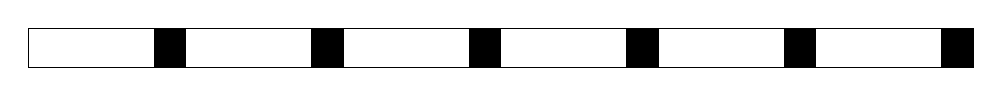
\begin{tikzpicture}[x=2cm,y=0.5cm]
\foreach \x in {0,1,2,3,4,5}
{
	\draw (\x,0) rectangle(\x+1,1);
	\draw[fill=black] (\x+0.8,0) rectangle(\x+1,1);
}
\end{tikzpicture}
\end{center}
}

\end{frame}

\newcommand{\rad}{0.3}
\begin{frame}
\begin{center}
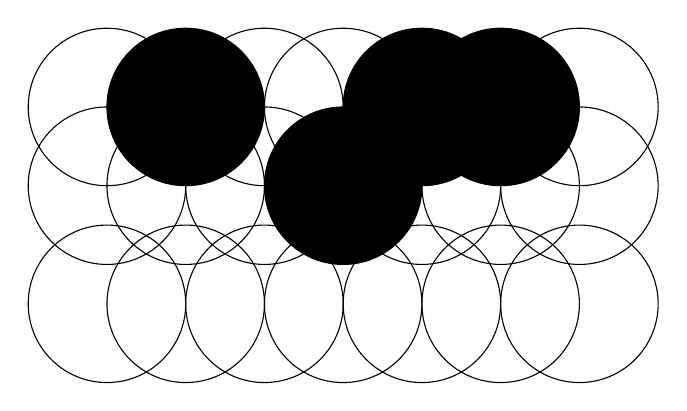
\begin{tikzpicture}[y=-1cm]
\uncover<+->{\draw (0,0) circle(\rad);
\draw[fill=black] (1,0) circle(\rad);
\draw (2,0) circle(\rad);
\draw (3,0) circle(\rad);
\draw[fill=black] (4,0) circle(\rad);
\draw[fill=black] (5,0) circle(\rad);
\draw (6,0) circle(\rad);

\draw (0,1) circle(\rad);
\draw (1,1) circle(\rad);
\draw (2,1) circle(\rad);
\draw[fill=black] (3,1) circle(\rad);
\draw (4,1) circle(\rad);
\draw (5,1) circle(\rad);
\draw (6,1) circle(\rad);}


\draw (0,2.5) circle(\rad);
\draw (1,2.5) circle(\rad);
\draw (2,2.5) circle(\rad);
\draw (3,2.5) circle(\rad);
\draw (4,2.5) circle(\rad);
\draw (5,2.5) circle(\rad);
\draw (6,2.5) circle(\rad);

\end{tikzpicture}
\end{center}

$$
S_1=6\cdot \frac{2}{3} = 4
$$

$$
S_2 = 6\cdot \left( \frac{2}{3}\cdot\frac{2}{3} + \frac{1}{3}\cdot\frac{1}{3} - \frac{2}{3}\cdot\frac{2}{3}\cdot\frac{1}{3}\cdot\frac{1}{3}\right)=6 \cdot \frac{41}{81} \approx 3.03 < 4
$$
\end{frame}

\begin{frame}
Байесовский фокус
\end{frame}

\end{document}